\section{Evaluation}\label{sec:evaluation}
\todo[inline]{Will need to rerun the benchmarks on a better machine, as Roulette is too slow and bit blast keeps timing out.}

This section confirms that the performance of \Slice{} is competitive with existing state-of-the-art exact and approximate inference solvers for hybrid probabilistic programs. In particular, we evaluate \Slice{} using Dice and Roulette backends against the exact inference solver SPPL~\cite{Saad2021SPPL} and the approximate inference solver HyBit~\cite{Garg2024BitBlast} on various benchmarks. Our evaluation consists of three sets of programs. First is a series of synthetic benchmarks designed to test the how well \Slice{} scales asymptotically compared to SPPL. Second is a set of benchmarks for verifying fairness properties of decision trees. Lastly, we evaluate \Slice{} on a series of small baseline programs commonly used to test PPLs in the literature. 

\subsection{Experimental Setup}\label{sec:experimenal-setup}
All experiments were run on a ..., using the original version of Dice (2020) from Holtzen et. al.~\cite{Holtzen2020Dice} and the most recent version of Roulette that uses Racket 8.13 and Rosette 4.1. Each experiment was carried out using a consistent-effort approach, with the goal of determining the most effective encoding for the program in each language and making sure that programs were equivalent across all languages. 

\subsection{Synthetic benchmarks}\label{sec:synthetic-benchmarks}
To evaluate the asymptotic performance of \Slice{}, we designed seven synthetic benchmarks that stress-test different variants of probabilistic programs with continuous distributions. Currently, there are no benchmarks in the literature that test scaling of continuous programs, and we seek to close this gap. Each benchmark generates programs that grow linearly in size in the number of comparison tests (e.g. number of $<$ operators) to measure how execution time scales. This bears resemblence to how scalability is tested for discrete PPLs in the litearture: by growing the program by adding one additional layer to the chain of \texttt{flips} that depends on the previous. Doing so results in a path enumeration that grows exponentially in the number of layers. We generate programs of varying structure:

\subsubsection{Conditional Independence.} 
If a variable \texttt{z} is conditionally independent of \texttt{x} given \texttt{y}, then \texttt{y} acts as a kind of interface between \texttt{x} and \texttt{z} that allows inference to be split into two separate analyses. Bayesian networks use conditional independence to compactly represent complex distributions, for example. We test programs where each variable's distribution depends on comparisons with previous variables, specifically when:

\begin{itemize}
\item Each variable depends on its immediate predecessor variable through conditional statements. This creates a chain of dependencies where $x_i$ depends on whether $x_{i-1} < c$ for some constant $c$. See Figure~\ref{fig:cond-benchmarks-a}.
\item Each variable depends on a randomly chosen predecessor variable through conditional statements. This creates a chain of dependencies where $x_i$ depends on whether $x_1, ..., x_{i-1}$ chosen uniformly at random is $< c$ for some constant $c$, but note this could lead to unused variables. See Figures~\ref{fig:cond-benchmarks-b} and~\ref{fig:cond-benchmarks-c}, where the former guarantees unique distributions for each variable whereas the latter generates random ones.
\end{itemize}

\begin{figure}[!t]
\centering
\begin{subfigure}{0.32\textwidth}
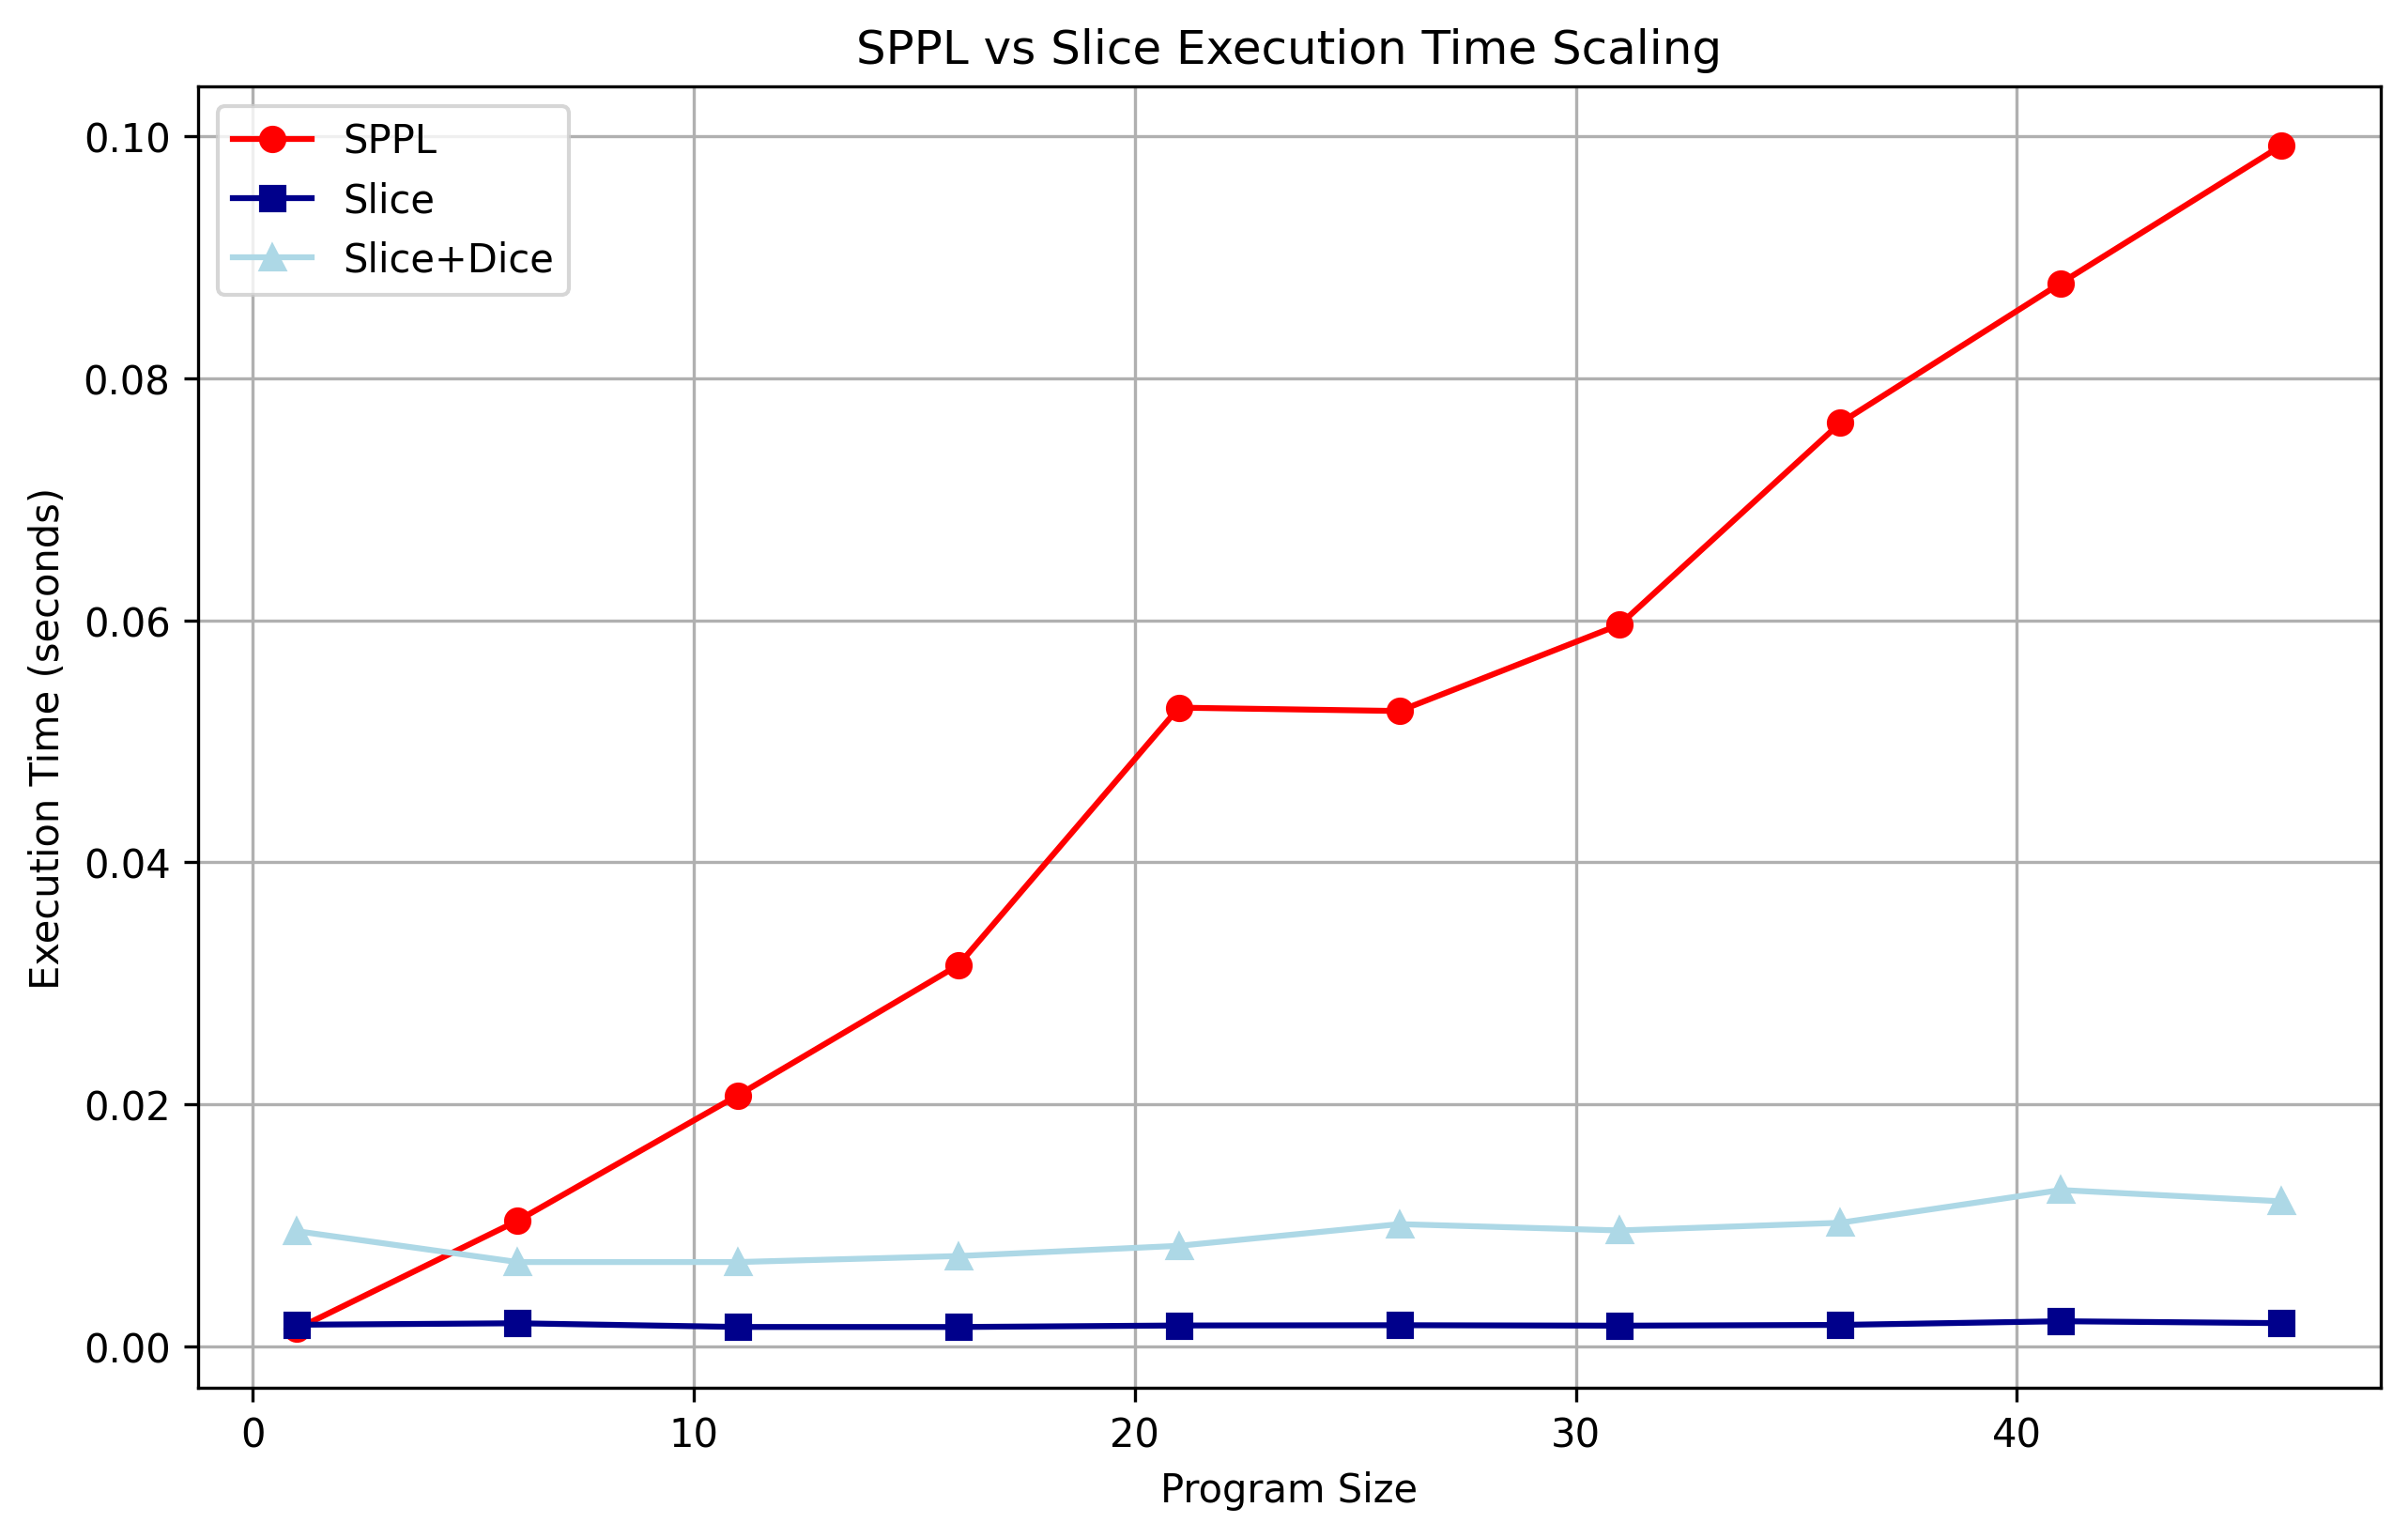
\includegraphics[width=\textwidth]{../images/scaling/build_conditional_independent_slice.png}
\caption{Conditional Independent}
\label{fig:cond-benchmarks-a}
\end{subfigure}
\hfill
\begin{subfigure}{0.32\textwidth}
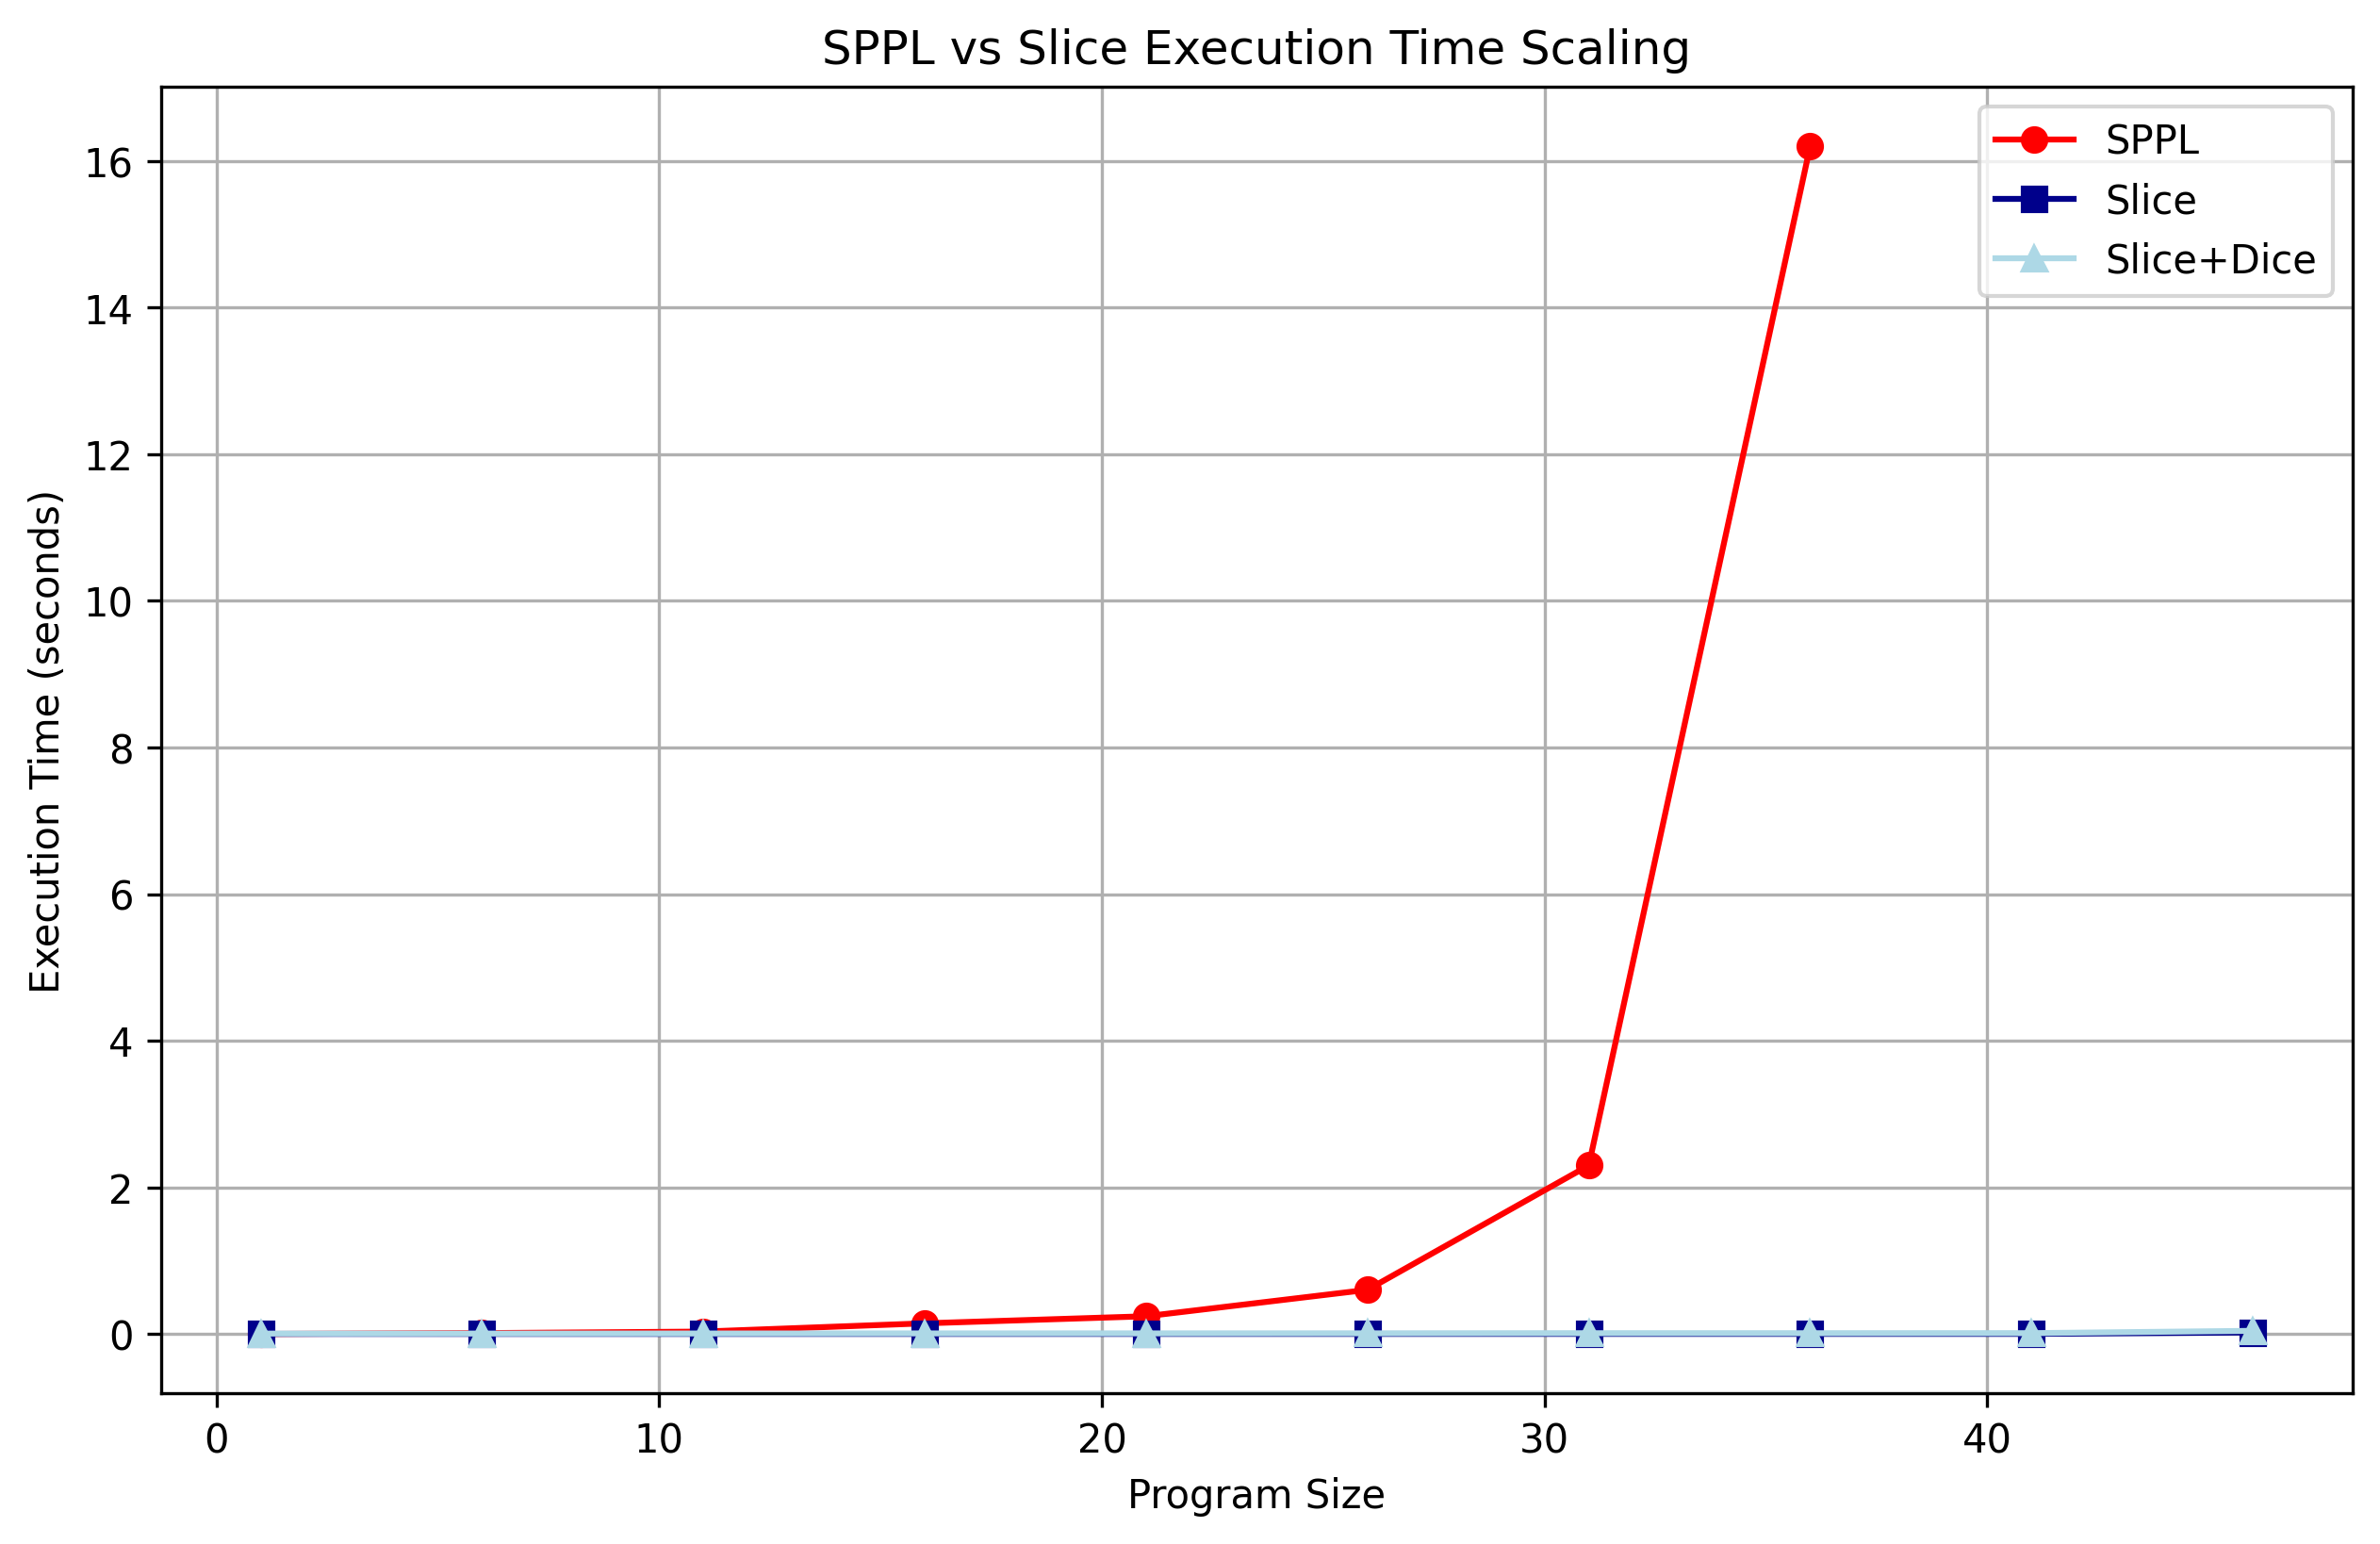
\includegraphics[width=\textwidth]{../images/scaling/build_conditional_random_independent_slice_1.png}
\caption{Conditional Random 1}
\label{fig:cond-benchmarks-b}
\end{subfigure}
\hfill
\begin{subfigure}{0.32\textwidth}
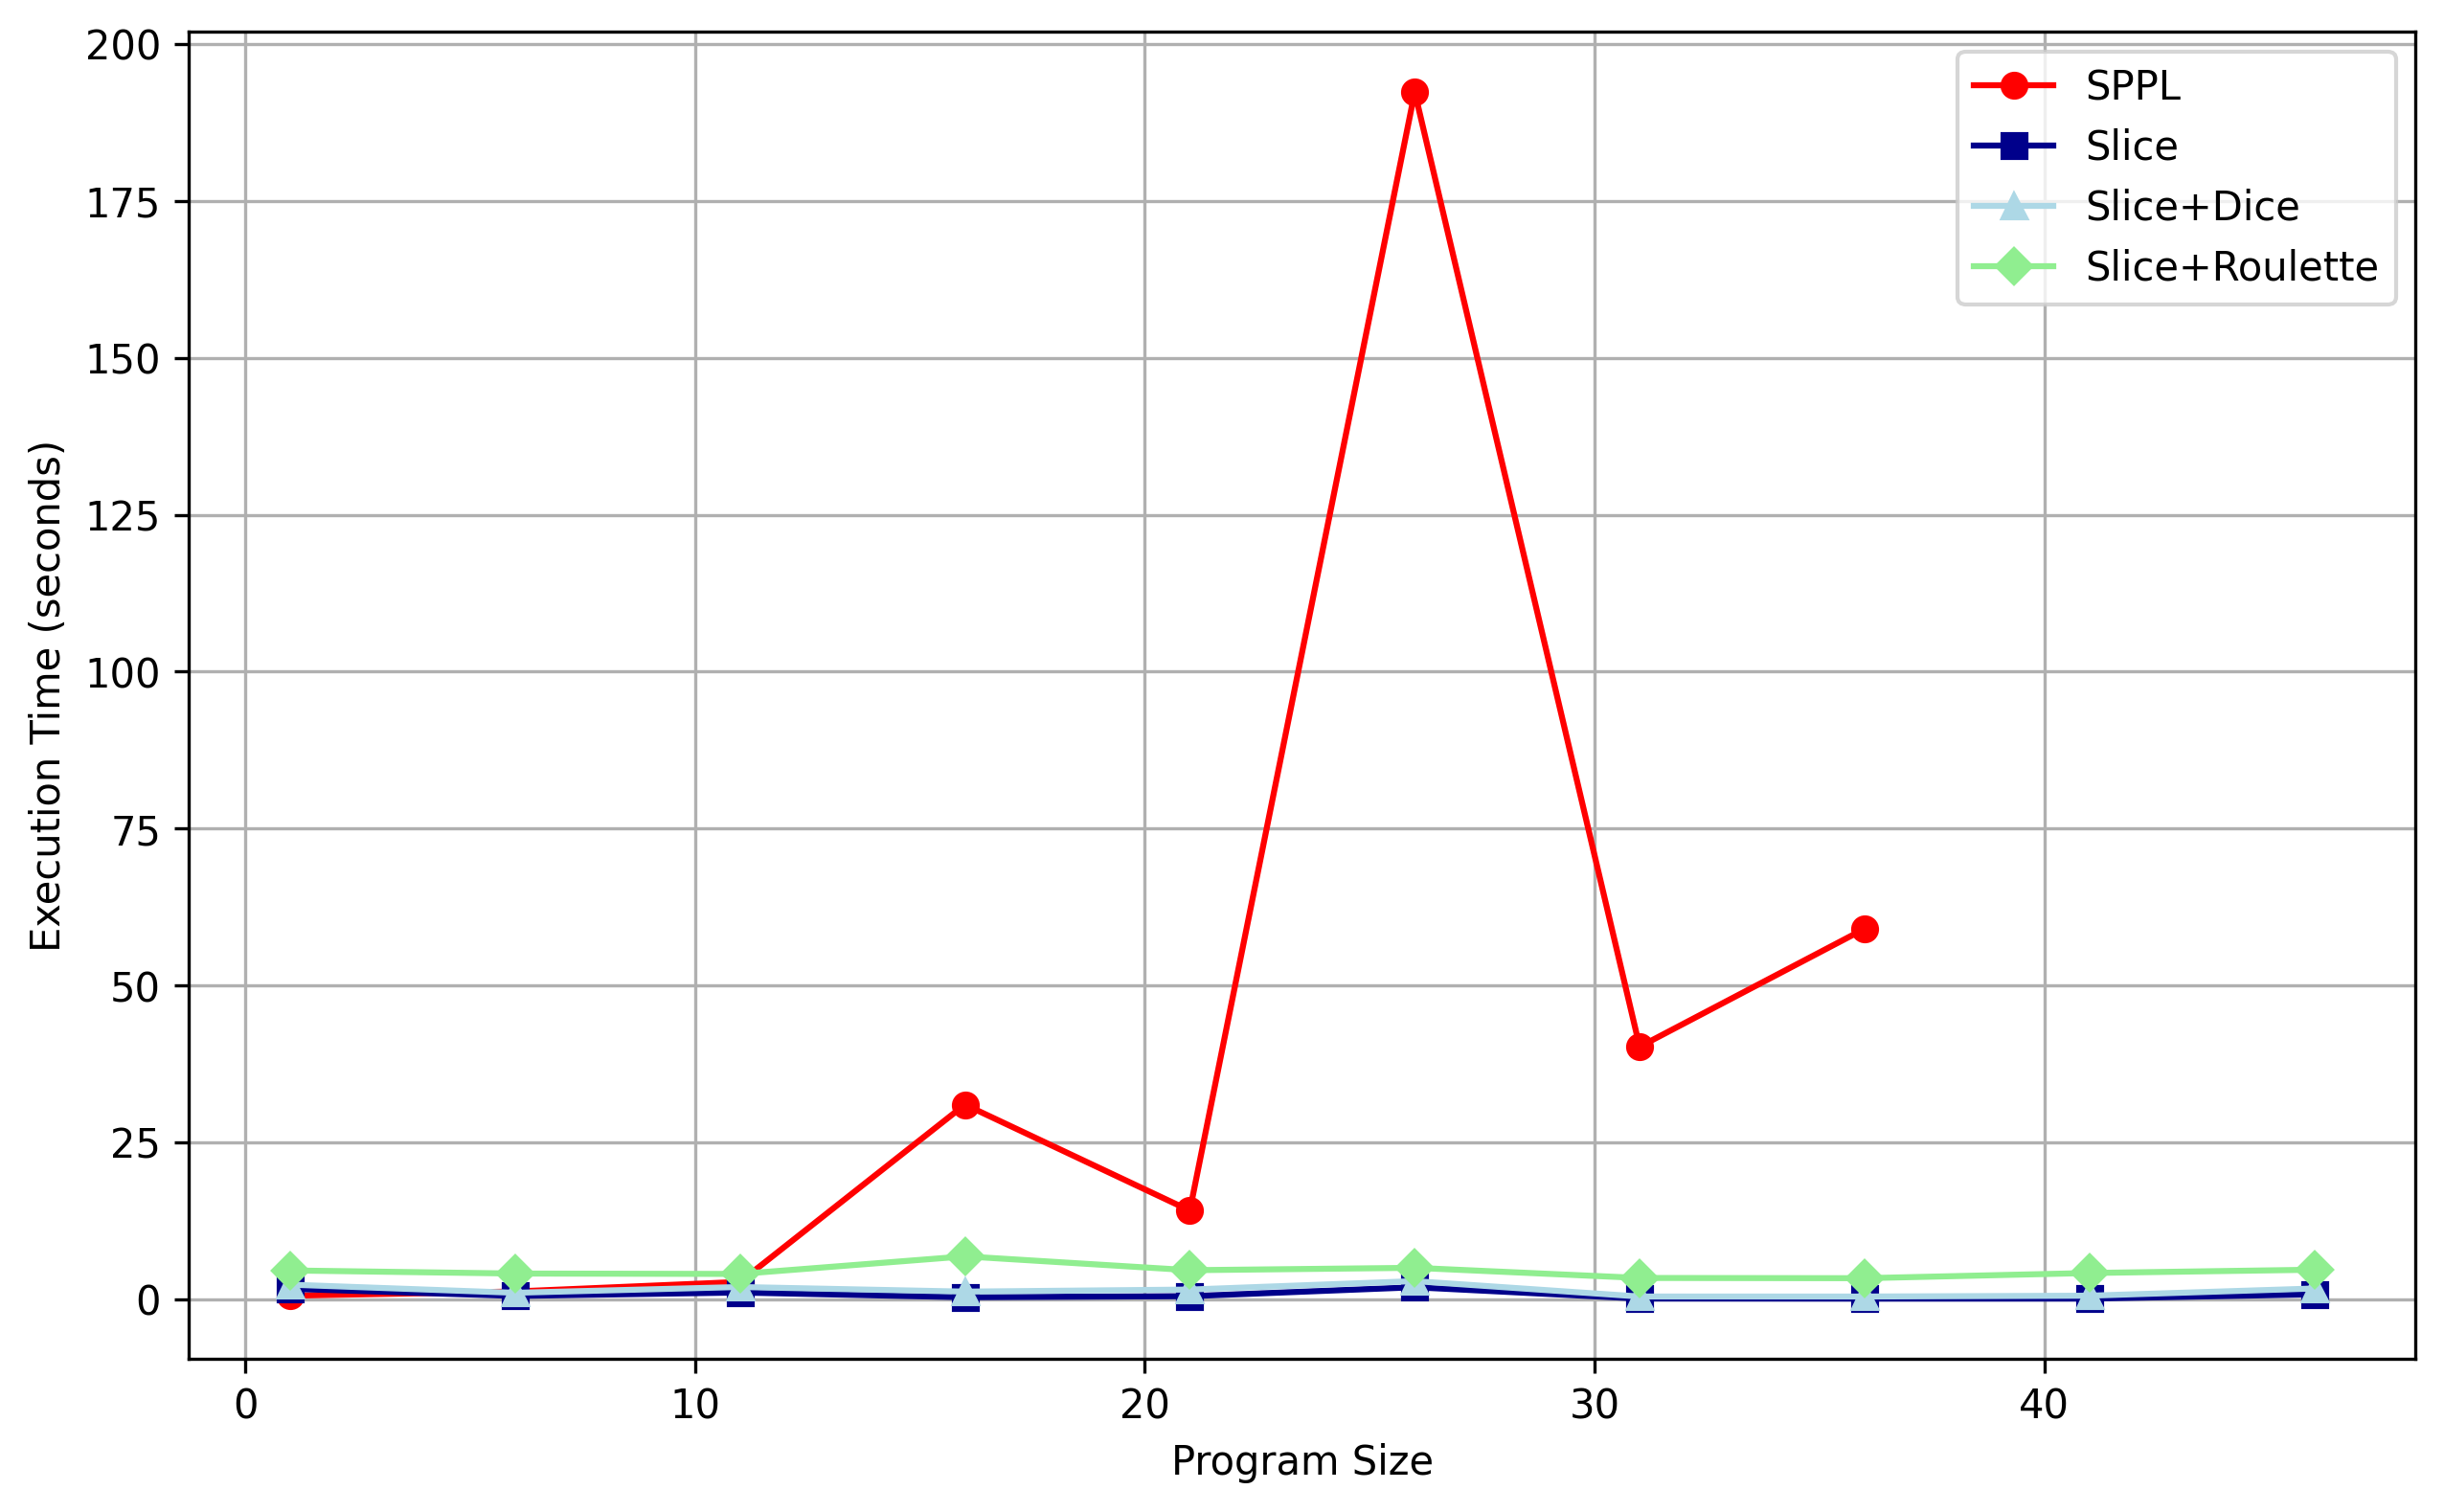
\includegraphics[width=\textwidth]{../images/scaling/build_conditional_random_independent_slice_2.png}
\caption{Conditional Random 2}
\label{fig:cond-benchmarks-c}
\end{subfigure}
\caption{Scaling results for conditional independence benchmarks. SPPL (red) shows exponential growth and times out early, while Slice (blue), Slice+Dice (light blue), and Slice+Roulette (light green) maintain near-linear scaling.}
\label{fig:cond-benchmarks}
\end{figure}

\subsubsection{Alternating Guards.}
We test programs with alternating comparison patterns,
where the control flow depends on earlier random variables. This pattern is characteristic of hierarchical or history-dependent probabilistic programs. Specifically, we test when:

\begin{itemize}
\item Variables in conditionals alternate based on a guard span parameter. For example, with span 3, guards cycle through $x_1, x_2, x_3, x_1, x_2, x_3, ...$ See Figure~\ref{fig:alt-benchmarks-a}. Since such programs may have unused variables, we remedy this by generating programs whose if-else bodies depend on the immediate predecessor variable; see Figures~\ref{fig:alt-benchmarks-b} and~\ref{fig:alt-benchmarks-c}.

\item Variables in conditionals alternate based on a guard span parameter, but we randomly choose the guard span parameter in each iteration instead of it being deterministically chosen as before. See Figure~\ref{fig:alt-benchmarks-d}.
\end{itemize}

\begin{figure}[!t]
\centering
\begin{subfigure}{0.48\textwidth}
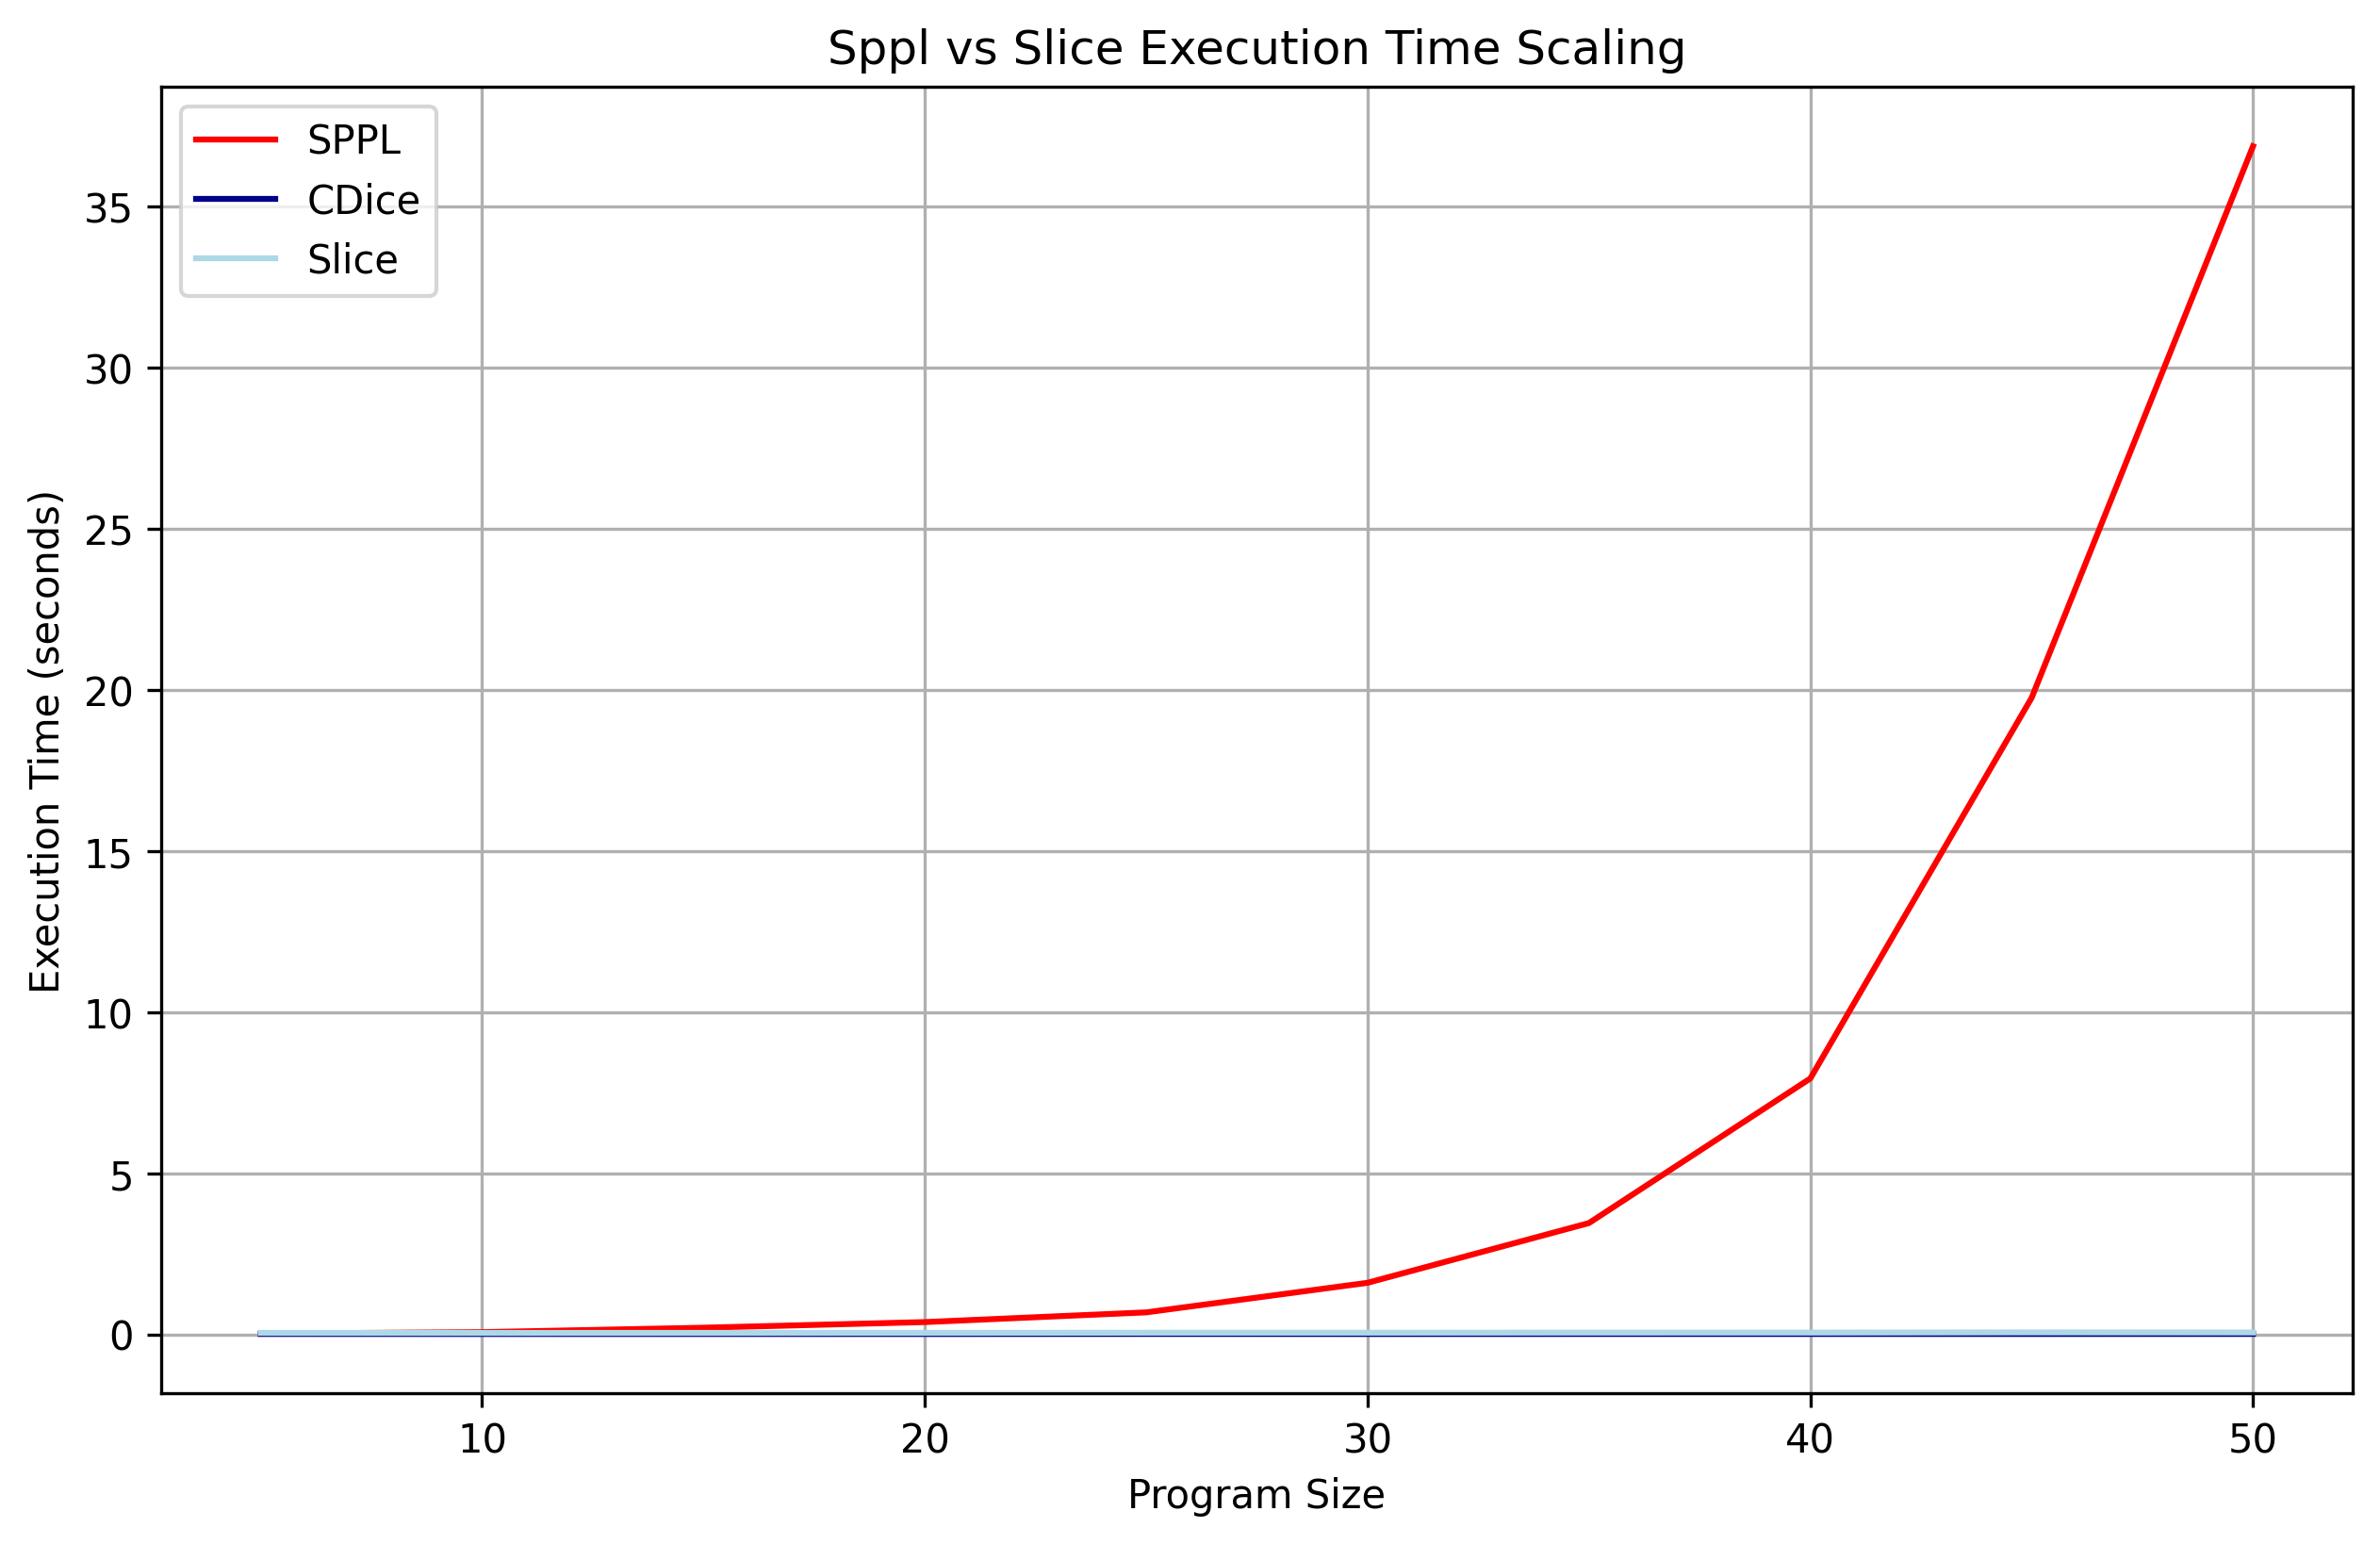
\includegraphics[width=\textwidth]{../images/scaling/build_alternating_guard_contdice_1.png}
\caption{Alternating Guard 1}
\label{fig:alt-benchmarks-a}
\end{subfigure}
\hfill
\begin{subfigure}{0.48\textwidth}
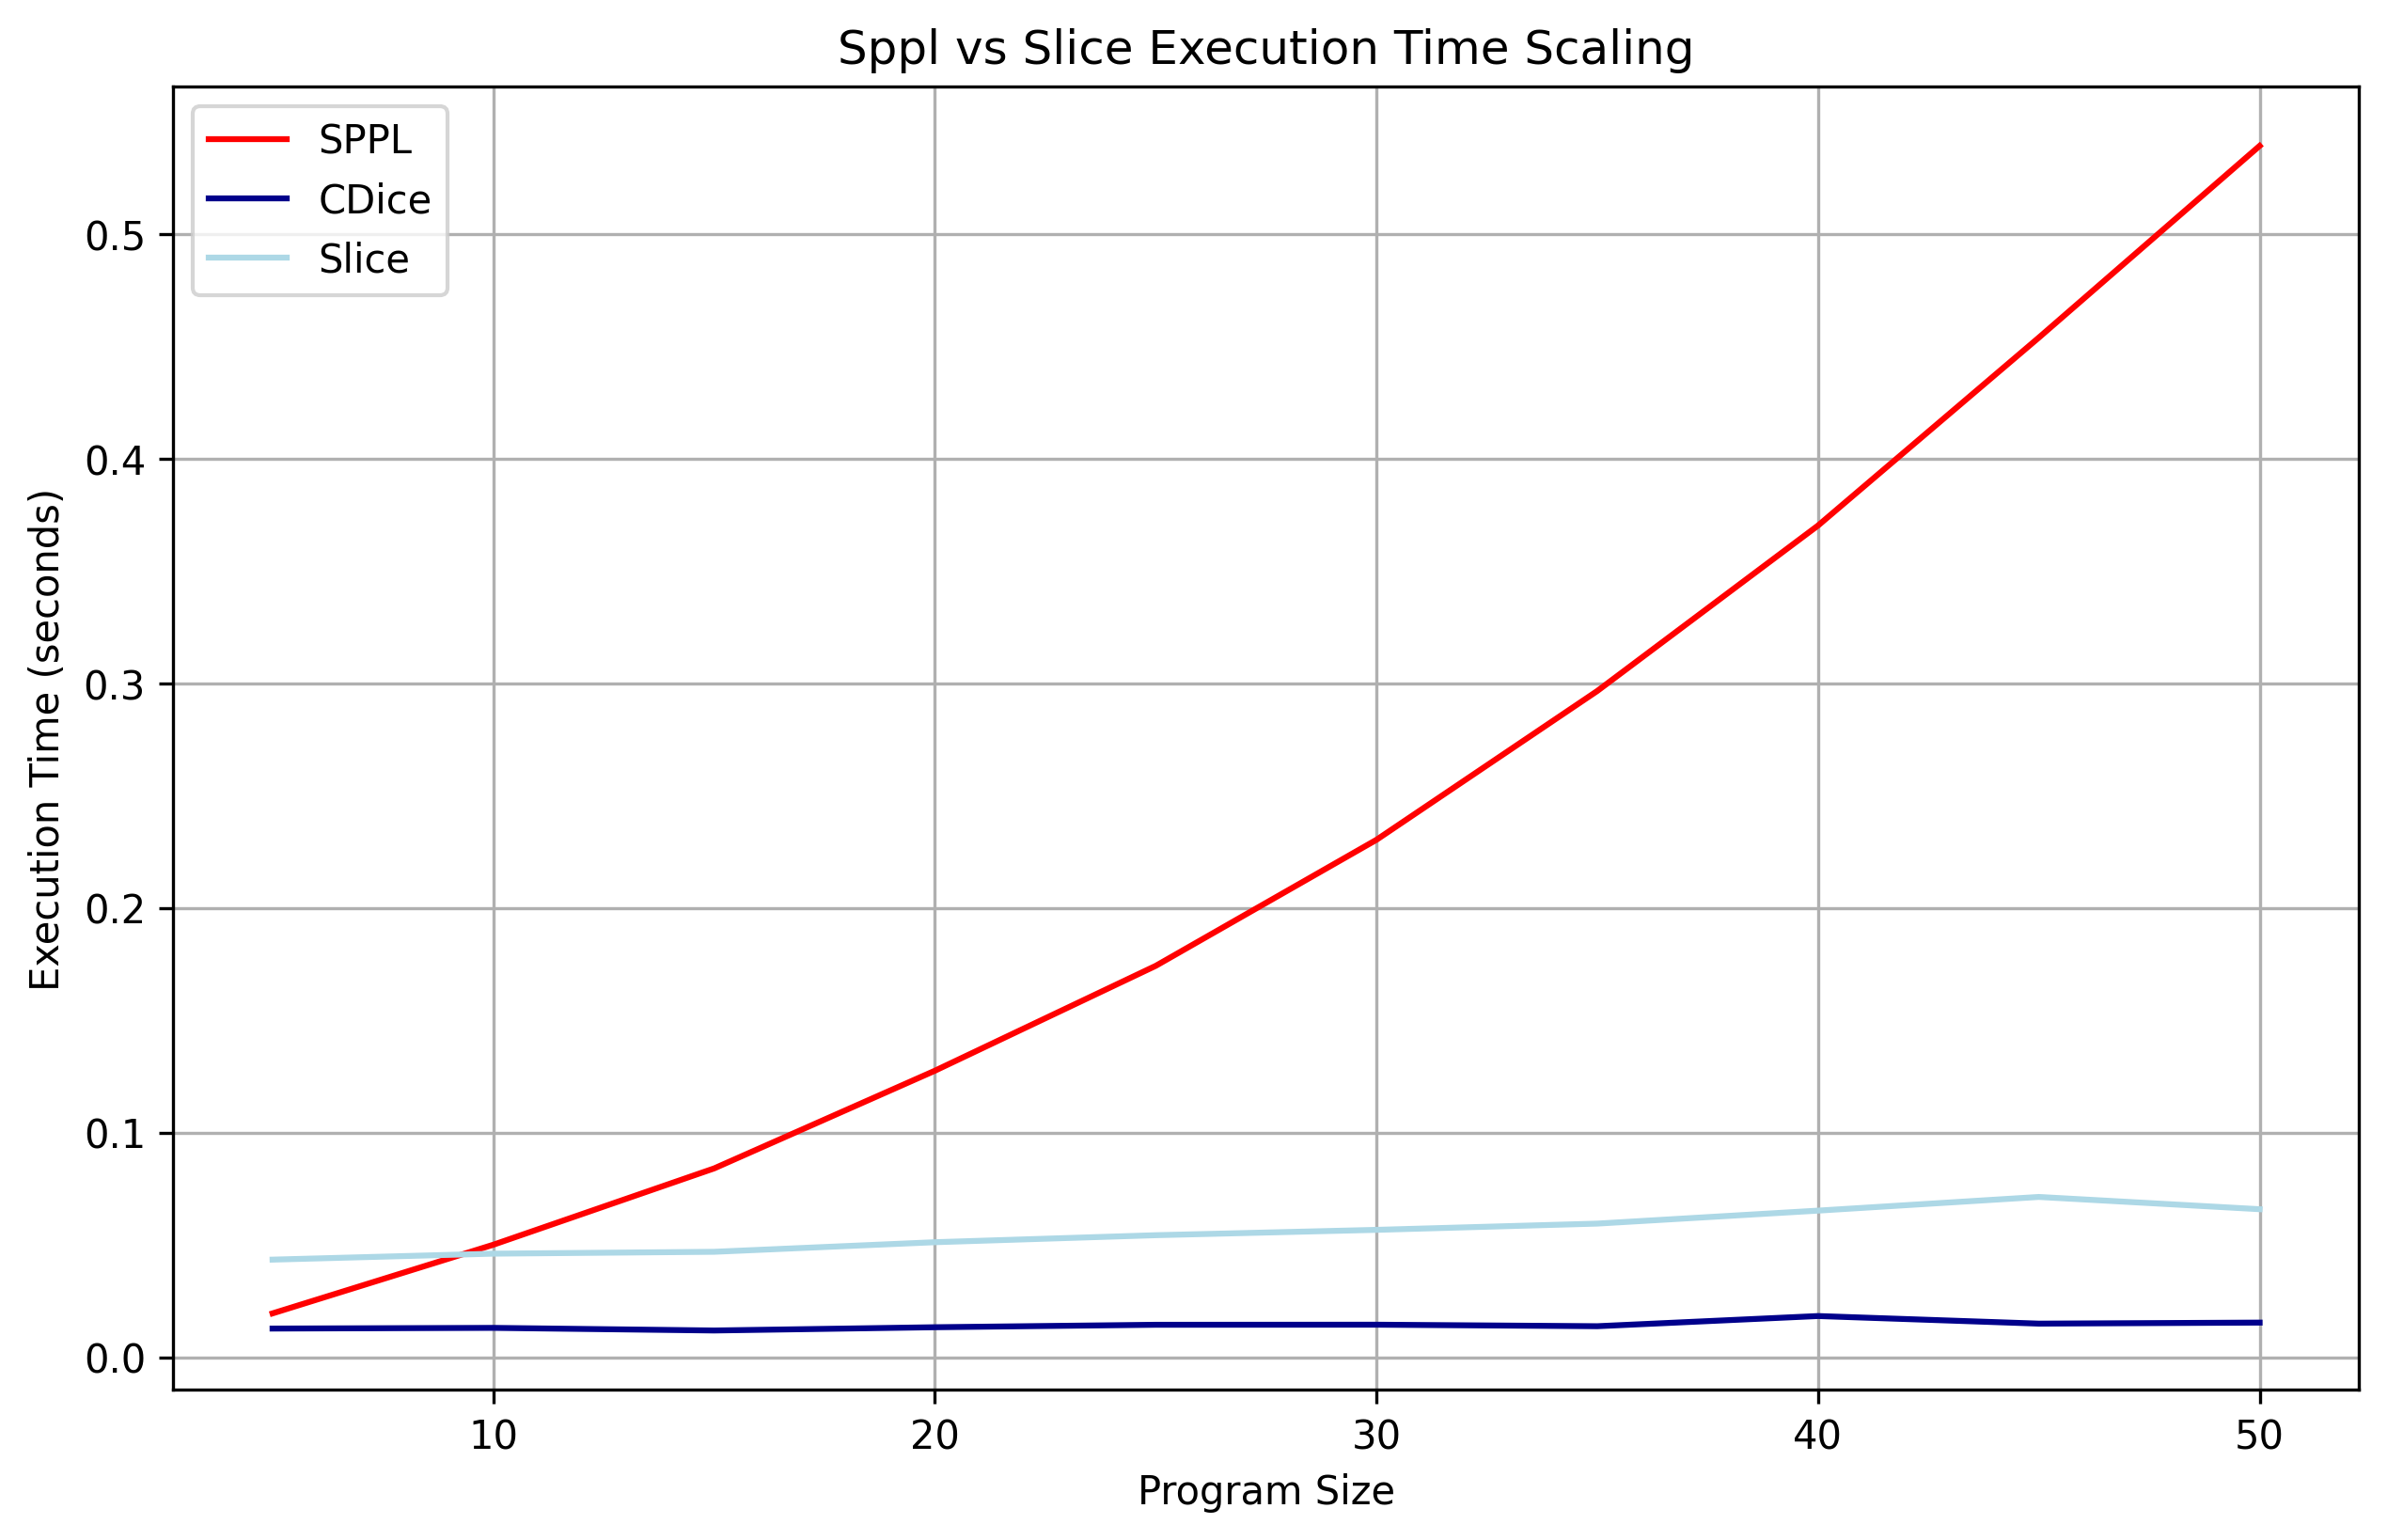
\includegraphics[width=\textwidth]{../images/scaling/build_alternating_guard_contdice_2.png}
\caption{Alternating Guard 2}
\label{fig:alt-benchmarks-b}
\end{subfigure}
\vspace{0.5em}
\begin{subfigure}{0.48\textwidth}
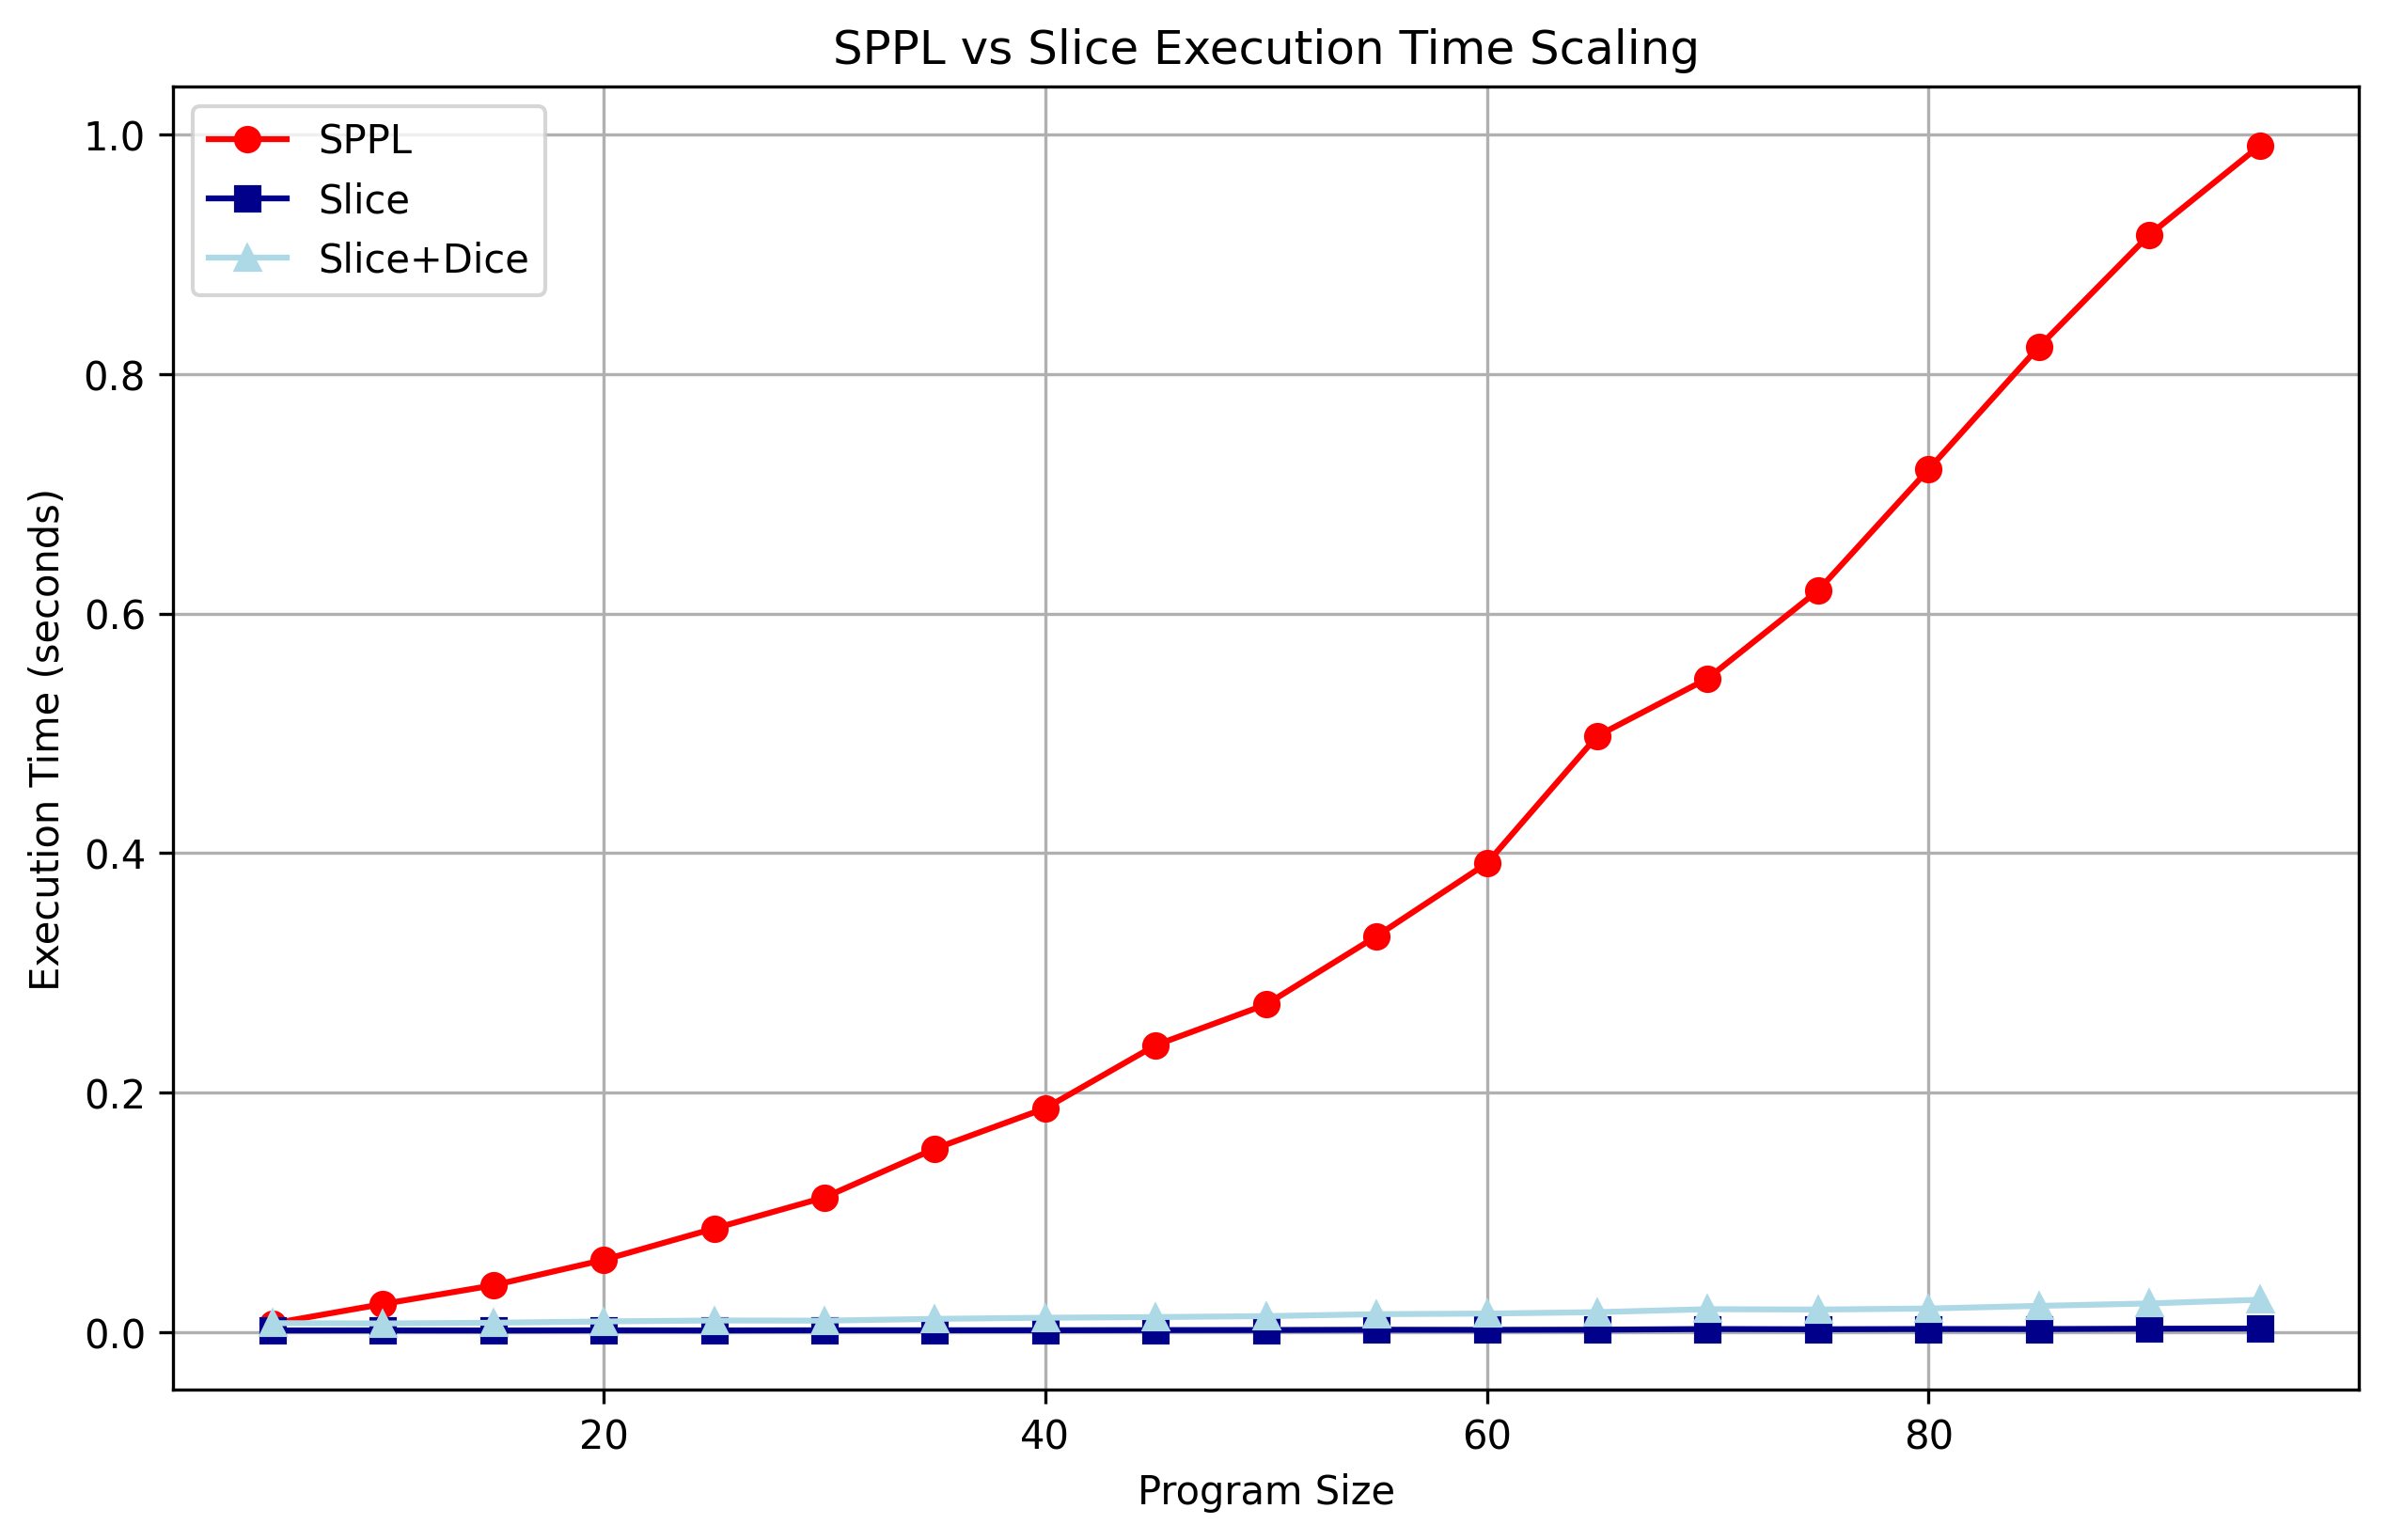
\includegraphics[width=\textwidth]{../images/scaling/build_alternating_guard_contdice_3.png}
\caption{Alternating Guard 3}
\label{fig:alt-benchmarks-c}
\end{subfigure}
\hfill
\begin{subfigure}{0.48\textwidth}
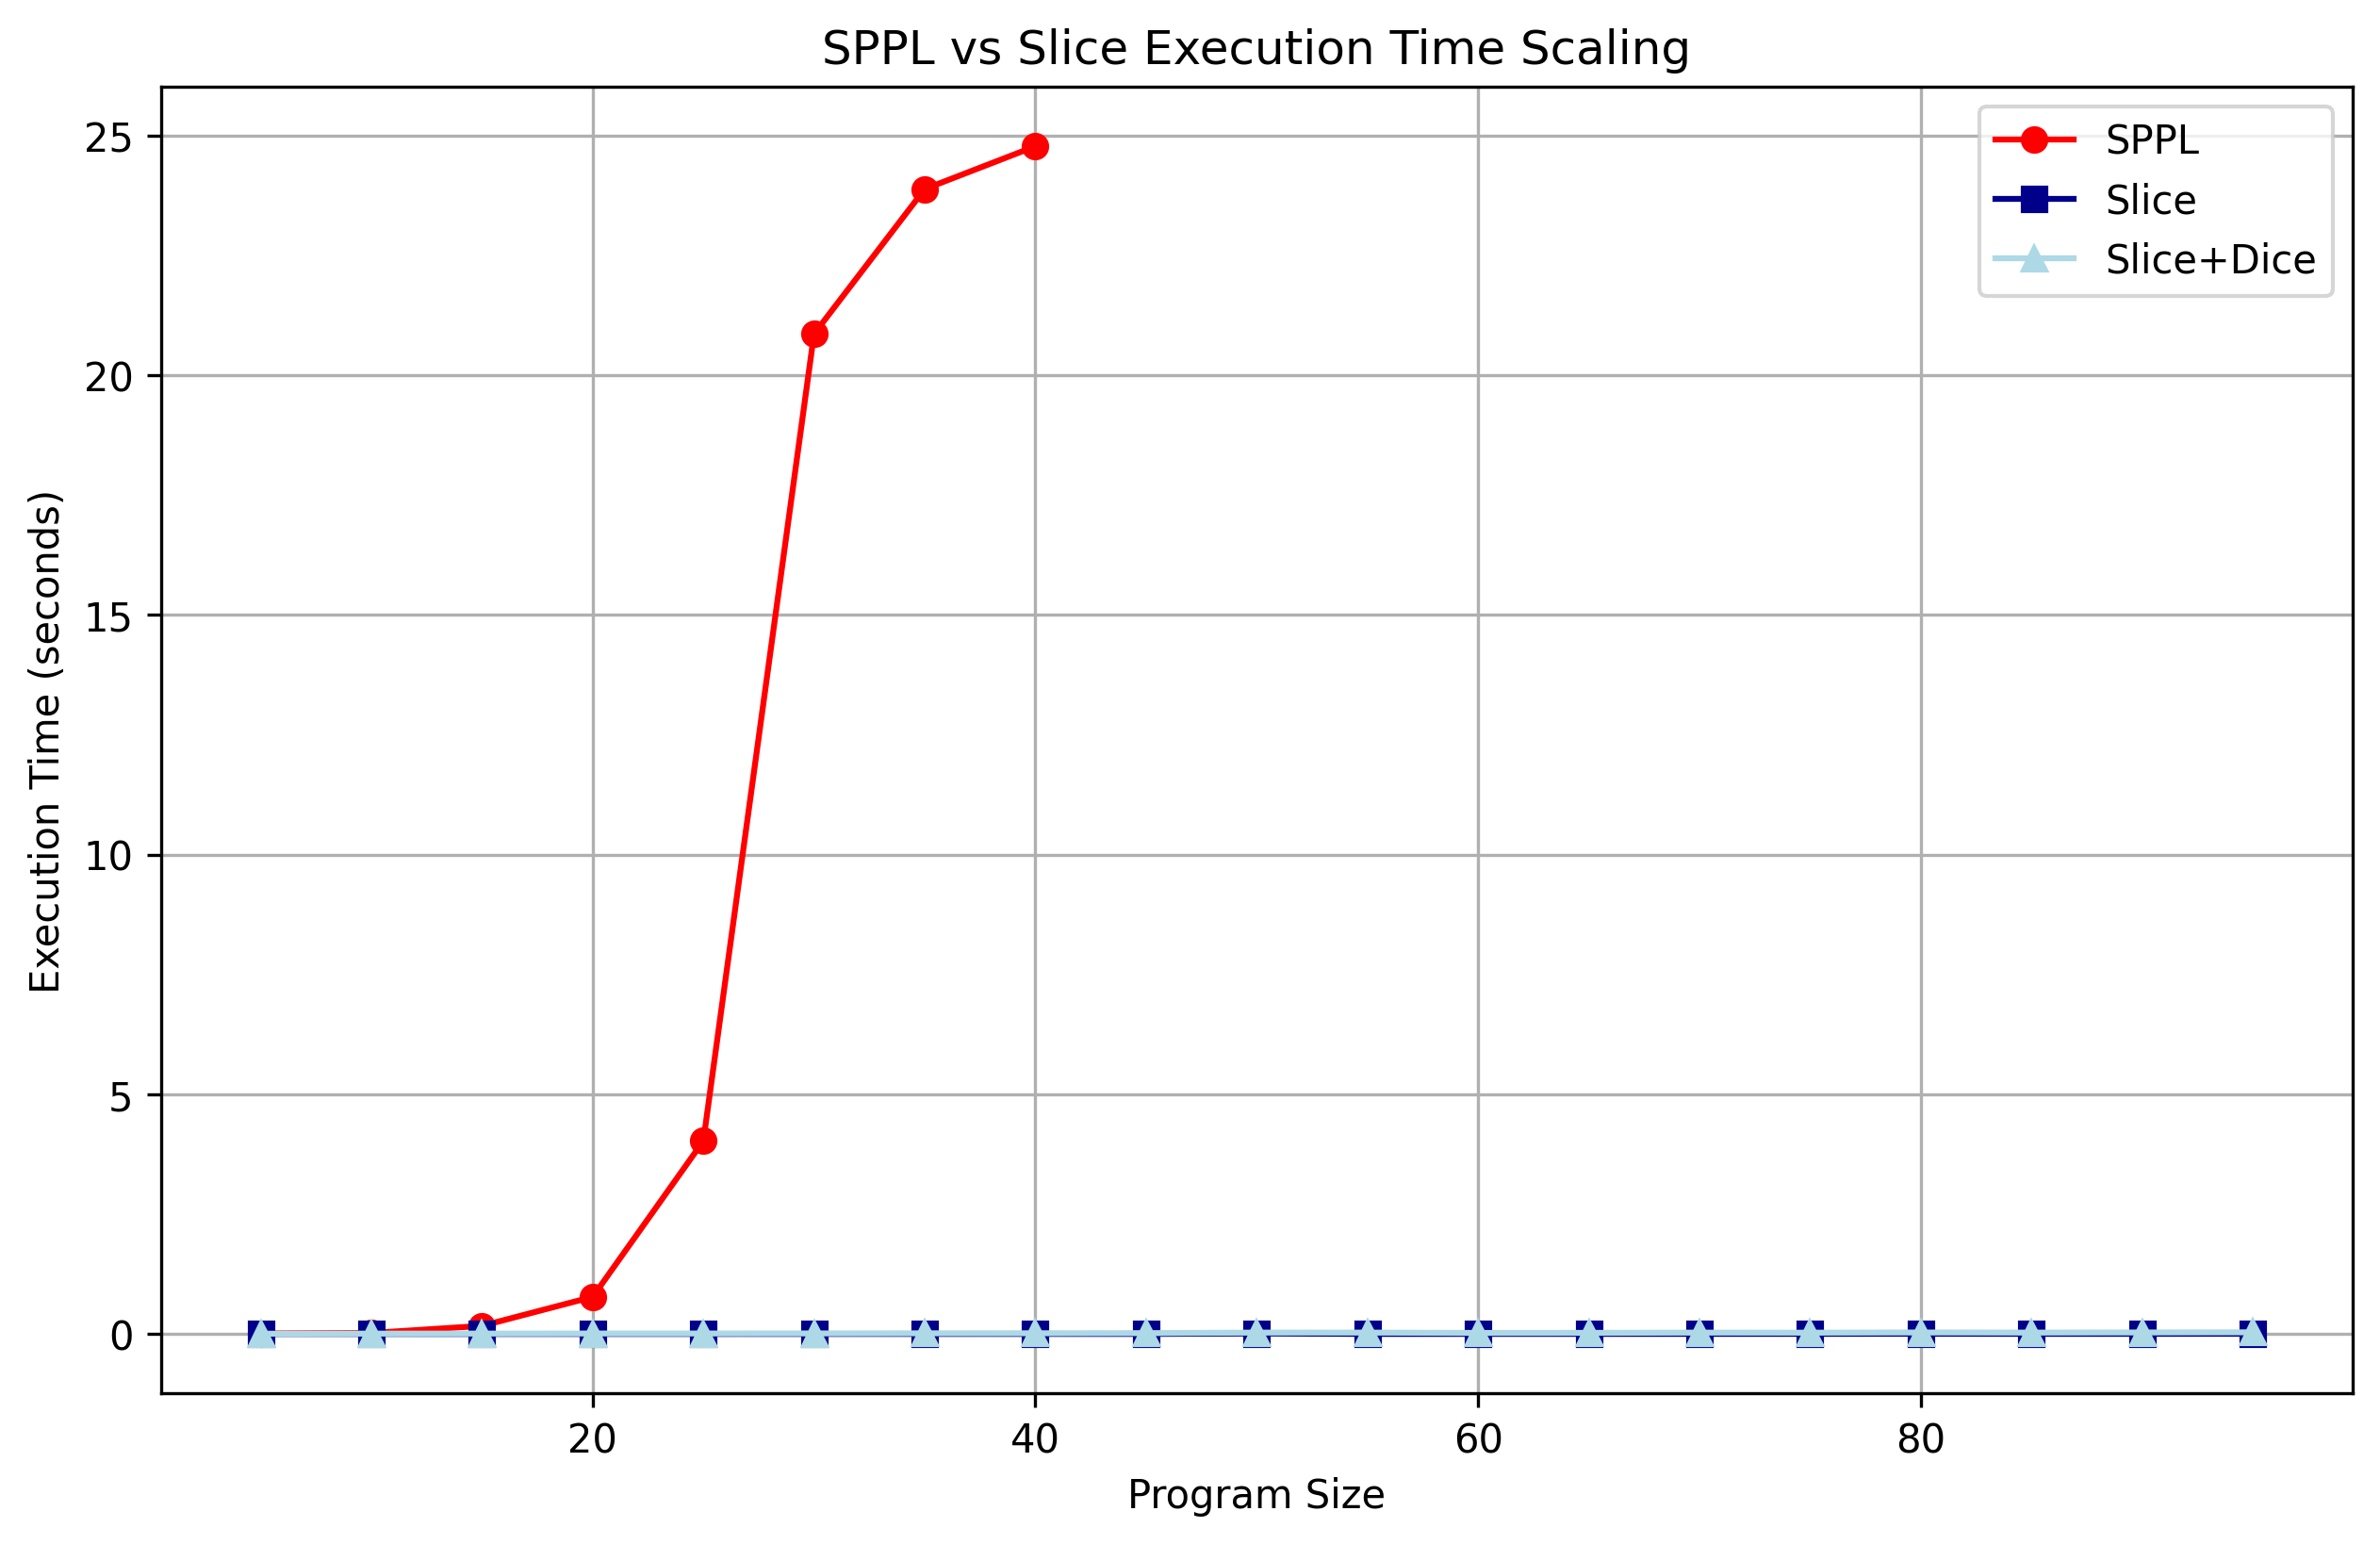
\includegraphics[width=\textwidth]{../images/scaling/build_random_alternating_guard_contdice.png}
\caption{Random Alternating Guard}
\label{fig:alt-benchmarks-d}
\end{subfigure}
\caption{Scaling results for alternating guard benchmarks. SPPL (red) times out early (between program sizes 20-30), while Slice continues to scale to large programs.}
\label{fig:alt-benchmarks}
\end{figure}

\paragraph{Results.} We generate programs of size 1-50 with step size 5 in each iteration for the conditional independence tests, and for the alternating guards tests, we generate programs of size 1-100 with step size 5 and 1 for the program size and guard span, respectively. We specify a timeout of 300s. The scaling experiments demonstrate that Slice maintains near-linear scaling behavior while SPPL exhibits significantly faster growth and times out on larger programs. Across all seven benchmarks, Slice+Dice execution time remains under 0.5 seconds even for programs with 90+ comparisons, while SPPL times out (at 300s) for programs as small as 20-30 in size. The Slice compilation phase alone (dark blue line) shows essentially constant time, indicating that the type-directed discretization algorithm scales extremely well.

\subsection{Fairness Benchmarks}\label{sec:fairness-benchmarks}
Characterizing the fairness of classification algorithms is an interesting application in machine learning~\cite{Dwork2012FairnessAwareness}. FairSquare~\cite{albarghouthi2017fairsquare} and VeriFair~\cite{Bastani2019VeriFair} are two solvers that obtain fairness judgments for large-scale decision-making programs. Prior to SPPL, they were state-of-the-art for verifying the fairness of decision tree classifiers, neural network classifiers, and support vector machine classifiers. We evaluate performance on the decision tree benchmarks, as \Slice cannot solve the neural network and support vector machine benchmarks as they contain multivariate transforms, and show that \Slice{} beats SPPL in performance on such benchmarks.

Table 1 shows the results. The first column shows the decision making program ($DT_n$ means ``decision tree'' with $n$ conditionals), and the remaining columns display the execution times in seconds of Slice with Dice, Slice with Roulette, and SPPL respectively. The last column measures the speedup of \Slice{} over SPPL, where we take the max between Dice and Roulette speedups. The measurements indicate that SPPL consistently obtains probability estimates in milliseconds, with up to about 200x in speedup compared to SPPL. Although FairSquare and VeriFair can compute approximate probabilities that enable them to express more fairness problems, their cost is that their runtime on the decision trees is higher and less predictable than \Slice{} and SPPL which can compute exact probabilities efficiently.

\begin{table}[!t]
\centering
\begin{tabular}{lrrrr}
\toprule
Benchmark & Slice+Dice (s) & Slice+Roulette (s) & SPPL (s) & Speedup \\
\midrule
DT4\_bn1 & 0.211 & 2.726 & 3.406 & 16.2× \\
DT4\_bn2 & 0.212 & 2.742 & 3.465 & 16.3× \\
DT4\_ind & 0.197 & 2.665 & 3.306 & 16.8× \\
DT14\_bn1 & 0.232 & 2.929 & 3.547 & 15.3× \\
DT14\_bn2 & 0.232 & 2.925 & 4.055 & 17.5× \\
DT14\_ind & 0.215 & 2.743 & 3.365 & 15.7× \\
DT16\_bn1 & 0.227 & 2.952 & 3.667 & 16.2× \\
DT16\_bn2 & 0.230 & 3.064 & 3.624 & 15.8× \\
DT16\_ind & 0.213 & 2.848 & 3.517 & 16.5× \\
DT44\_bn1 & 0.273 & 3.806 & 3.967 & 14.5× \\
DT44\_bn2 & 0.277 & 3.586 & 3.934 & 14.2× \\
DT44\_ind & 0.243 & 3.067 & 3.686 & 15.1× \\
\bottomrule
\end{tabular}
\caption{Execution times (seconds) for decision tree benchmarks}
\end{table}

\subsection{Simple Baselines}\label{sec:baseline-benchmarks}
We finally evaluate \Slice{} on a set of benchmarks that were introduced by~\cite{gehr2016psi}. We evaluate \Slice{} on the hybrid programs in these benchmarks. The results are shown in Table 2. We omit the runs of PSI in the table due to its significally slower performance than SPPL on all benchmarks. The first column in the table gives the benchmark name, and the remaining columns display the execution times in seconds of Slice with Dice, Slice with Roulette, and SPPL respectively. As both SPPL and \Slice{} are restricted languages, in order to test a broader range of programs, we converted several benchmarks with parameters inside distributions that depend on continuous random choices to a discretized version. The time taken by \Slice{} to solve these problems is nearly instant in all cases. 

\begin{table}[!t]
\centering
\begin{tabular}{lrrrr}
\toprule
Benchmark & Slice+Dice (s) & Slice+Roulette (s) & SPPL (s) & Speedup \\
\midrule
ClickGraph & 0.510 & 4.891 & 109.868 & 215.4× \\
ClinicalTrial & 0.738 & 4.352 & 7.965 & 10.8× \\
CoinBias & 0.261 & 3.006 & 4.067 & 15.6× \\
SurveyUnbias & 0.229 & 2.849 & 3.599 & 15.7× \\
TrueSkill & 0.222 & 2.762 & 3.438 & 15.4× \\
\bottomrule
\end{tabular}
\caption{Execution times for clinical trial benchmark}
\end{table}